% SIPAIM 2026 -- TEM Axon & Myelin Segmentation Challenge: method description
% IEEE conference template (IEEEtran). Max. 4 pages + 1 page for references only.
% Review is single-blind: authors and affiliations must be included.
\documentclass[conference]{IEEEtran}
\IEEEoverridecommandlockouts

\usepackage{cite}
\usepackage{amsmath,amssymb}
\usepackage{graphicx}
\usepackage{booktabs}
\usepackage{xcolor}
\usepackage{url}

\begin{document}

\title{Paired Axon--Myelin Instance Segmentation in TEM\\
with Fine-Tuned Cellpose-SAM and Recall-Oriented Multi-Scale Inference}

% TODO: completar autores, afiliaciones y correos (revisión single-blind: son obligatorios)
\author{
\IEEEauthorblockN{Author One\IEEEauthorrefmark{1},
Author Two\IEEEauthorrefmark{1},
Author Three\IEEEauthorrefmark{2}}
\IEEEauthorblockA{\IEEEauthorrefmark{1}Department, Institution, City, Country}
\IEEEauthorblockA{\IEEEauthorrefmark{2}Department, Institution, City, Country\\
Email: \{author.one, author.two\}@institution.edu}
}

\maketitle

\begin{abstract}
The g-ratio, the ratio between the inner axonal and the outer fiber diameter, is
a key biomarker of myelination, and computing it per fiber requires instance
segmentation of every axon \emph{paired} with its myelin sheath. We address the
TEM Axon \& Myelin Segmentation Challenge with two fine-tuned Cellpose-SAM
models, one for whole fibers and one for axons, combined so that the myelin
sheath is the fiber minus its axon; the axon/myelin pairing is therefore
guaranteed by construction, and fibers merged by the network are split by
nearest-axon assignment. An oracle-based error analysis on a held-out
validation set shows that the 95th-percentile Hausdorff distance (HD95) is
dominated by whole fibers that are never detected (14\% of the annotated
fibers), not by boundary errors, whose median IoU is 0.966. We therefore adopt a
recall-oriented inference that lowers the cell-probability threshold and adds a
second pass at half scale. Without retraining, it improves the mean Dice from
0.828 to 0.865, the HD95 from 669 to 535~nm and the g-ratio mean absolute error
from 0.0167 to 0.0151 on 39 validation images.
\end{abstract}

\begin{IEEEkeywords}
transmission electron microscopy, axon, myelin, instance segmentation, g-ratio, Cellpose-SAM
\end{IEEEkeywords}

% =====================================================================
\section{Introduction}

Quantitative morphometry of myelinated axons in transmission electron
microscopy (TEM) is central to the study of demyelinating and
neurodegenerative disorders. The most widely used biomarker is the g-ratio,
$g = D_{\text{axon}} / D_{\text{fiber}}$, whose optimal value has been studied
theoretically for the central nervous system~\cite{chomiak2009}. Measuring it
for every fiber requires more than semantic segmentation: each axon must be
delineated as an individual instance and linked to its own myelin sheath.

Deep-learning tools such as AxonDeepSeg~\cite{zaimi2018} segment axon and
myelin semantically and recover instances in post-processing, and
self-configuring U-Nets such as nnU-Net~\cite{isensee2021} are strong semantic
baselines. Densely packed, touching fibers make the semantic-to-instance step
error-prone. Cellpose~\cite{stringer2021} instead predicts instances directly
through spatial flow fields, and its latest version, Cellpose-SAM~\cite{pachitariu2025},
pairs this formulation with a Segment Anything (SAM)~\cite{kirillov2023}
vision-transformer encoder.

Our contributions are: (i) a two-model Cellpose-SAM formulation (fibers and
axons) whose combination always yields valid axon/myelin pairs; (ii) an
oracle-based decomposition of the validation error showing that missed whole
fibers, not boundary inaccuracy, dominate the HD95; and (iii) a recall-oriented,
multi-scale inference that improves all challenge metrics without retraining.

% =====================================================================
\section{Data and Evaluation}

The challenge provides 266 annotated TEM images of the mouse corpus callosum
(8-bit, $3008\times4096$ pixels, 2.152~nm/pixel). Labels are 16-bit instance
maps: 0 is background, 1 marks artifacts (excluded from every metric), an even
value $X\geq2$ is an axon and $X+1$ is its myelin sheath.

The challenge metrics are: the Dice similarity coefficient (DSC) of the axon
compartment (all even labels) and of the myelin compartment (all odd labels
$\geq3$); the HD95 of each compartment, defined as the maximum of the two
directed 95th percentiles of boundary-to-boundary distances, converted to nm;
and the mean absolute error of the per-fiber g-ratio (MAE$_g$), with
$D = 2\sqrt{A/\pi}$ computed from the axon area and the fiber ($X \cup X+1$)
area, over predicted fibers matched to ground-truth fibers by IoU. We
implemented these definitions and report the DSC and HD95 averaged over images
(mean of the two compartments) and MAE$_g$ pooled over all matched fibers.
We held out 39 randomly selected images (15\%, 1094 annotated fibers) for
validation and trained on the remaining 227.

% =====================================================================
\section{Method}

\begin{figure*}[t]
\centering
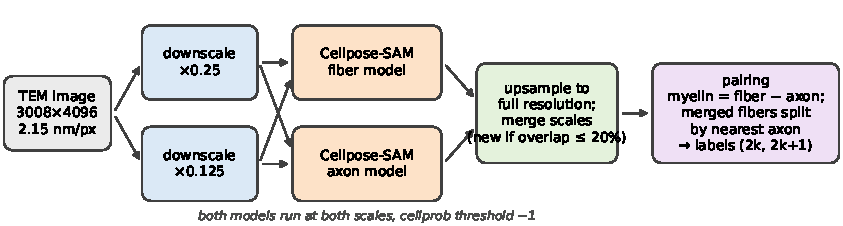
\includegraphics[width=0.92\textwidth]{figures/pipeline.pdf}
\caption{Inference pipeline. Two fine-tuned Cellpose-SAM models segment whole
fibers and axons at two scales; the instances are brought back to full
resolution, merged across scales and paired so that each axon $2k$ receives the
myelin sheath $2k+1$ of its own fiber.}
\label{fig:pipeline}
\end{figure*}

\subsection{Problem formulation}
Cellpose segments non-overlapping instances, whereas a fiber contains two
nested compartments. We therefore train two models on derived labels: a
\emph{fiber} model, where each instance is the union of an axon and its sheath
(label $\lfloor X/2 \rfloor$ for $X\geq2$), and an \emph{axon} model, where each
instance is an axon (even labels only). The myelin is recovered as the fiber
minus its axon (Fig.~\ref{fig:pipeline}). Because Cellpose has no ignore label,
artifact pixels are treated as background during training.

\subsection{Network and training}
Both models are initialized from the public Cellpose-SAM weights~\cite{pachitariu2025}:
a SAM ViT-L encoder~\cite{kirillov2023} (24 transformer blocks) followed by a
head that predicts the two flow components and a cell probability, from which
masks are obtained by gradient tracking~\cite{stringer2021}. Images are
downscaled by a factor of 0.25 ($752\times1024$) so that typical fibers
(equivalent diameter of about 350 pixels, i.e.\ 0.75~$\mu$m) fall within the size
range the model handles well. To reduce memory and preserve the pretrained
features, we freeze the patch and positional embeddings and the first 12
transformer blocks, leaving 152M of 305M parameters trainable. Each model is
trained for 200 epochs on random $256\times256$ crops with the default Cellpose
augmentation, AdamW~\cite{loshchilov2019} (learning rate $10^{-5}$, weight decay
0.1), batch size 4 and the default Cellpose schedule (linear warm-up and
step-wise decay in the last epochs). Training takes about 75~min per model on
a single 12~GB NVIDIA RTX 3080.

\subsection{Fiber/axon pairing}
Predicted instances are upsampled to full resolution with nearest-neighbour
interpolation. For each predicted fiber we collect the axon instances inside it
(at least 20 pixels). A fiber without an axon is discarded, since its g-ratio is
undefined. With one axon, the axon (holes filled) receives label $2k$ and the
rest of the fiber label $2k+1$. With several axons, the network has merged
touching fibers: every fiber pixel is assigned to its nearest axon (Euclidean
distance transform) and one pair is emitted per axon. Pairs whose myelin has
fewer than 20 pixels are dropped. The output is valid by construction: when fed
the ground-truth fiber and axon instances, this step reconstructs the reference
exactly (DSC 1, HD95 0~nm).

\subsection{Recall-oriented multi-scale inference}
\label{sec:inference}
Motivated by the analysis in Section~\ref{sec:analysis}, inference (i) lowers the
Cellpose cell-probability threshold from 0 to $-1$ and (ii) runs both models a
second time on the image downscaled by 0.125. A second-pass instance is added
only if at most 20\% of its area overlaps already detected instances; pairing
is applied afterwards. Inference takes about 12~s per image.

% =====================================================================
\section{Error Analysis}
\label{sec:analysis}

\begin{table}[t]
\caption{Oracle analysis on the validation set (Cellpose default inference).
Each row corrects one error type using the ground truth.}
\label{tab:oracle}
\centering
\small
\setlength{\tabcolsep}{3.5pt}
\begin{tabular}{@{}lccc@{}}
\toprule
Setting & DSC $\uparrow$ & HD95 (nm) $\downarrow$ & MAE$_g$ $\downarrow$ \\
\midrule
Default inference              & 0.828 & 669 & 0.0167 \\
$-$ background false pos.      & 0.848 & 653 & 0.0167 \\
Perfect matched boundaries     & 0.869 & 659 & 0.0031 \\
$-$ false pos.\ $+$ missed fibers & 0.962 & 24 & 0.0099 \\
GT through $\times0.25$ scale  & 0.986 & 4 & 0.0011 \\
\bottomrule
\end{tabular}
\end{table}

\begin{table*}[t]
\caption{Validation results (39 images) of the same trained models with
different inference settings. DSC and HD95 are averaged over images; MAE$_g$ is
pooled over matched fibers.}
\label{tab:results}
\centering
\small
\begin{tabular}{@{}lccccccc@{}}
\toprule
 & \multicolumn{3}{c}{DSC $\uparrow$} & \multicolumn{3}{c}{HD95 (nm) $\downarrow$} & \\
\cmidrule(lr){2-4}\cmidrule(lr){5-7}
Inference & axon & myelin & mean & axon & myelin & mean & MAE$_g$ $\downarrow$ \\
\midrule
Cellpose defaults                              & 0.844 & 0.812 & 0.828 & 710 & 628 & 669 & 0.0167 \\
Flow-error check disabled                      & 0.860 & 0.815 & 0.837 & 611 & 539 & 575 & 0.0259 \\
Cell-probability threshold $-1$                & 0.874 & 0.837 & 0.856 & 563 & 527 & 545 & \textbf{0.0151} \\
Multi-scale ($\times0.25$ + $\times0.125$)     & 0.881 & 0.837 & 0.859 & 574 & \textbf{484} & \textbf{529} & 0.0163 \\
Multi-scale, threshold $-1$ on second pass     & 0.884 & 0.839 & 0.862 & 564 & 499 & 532 & 0.0173 \\
\textbf{Multi-scale, threshold $-1$ (ours)}    & \textbf{0.886} & \textbf{0.843} & \textbf{0.865} & \textbf{547} & 524 & 535 & \textbf{0.0151} \\
\bottomrule
\end{tabular}
\end{table*}

\begin{figure*}[t]
\centering
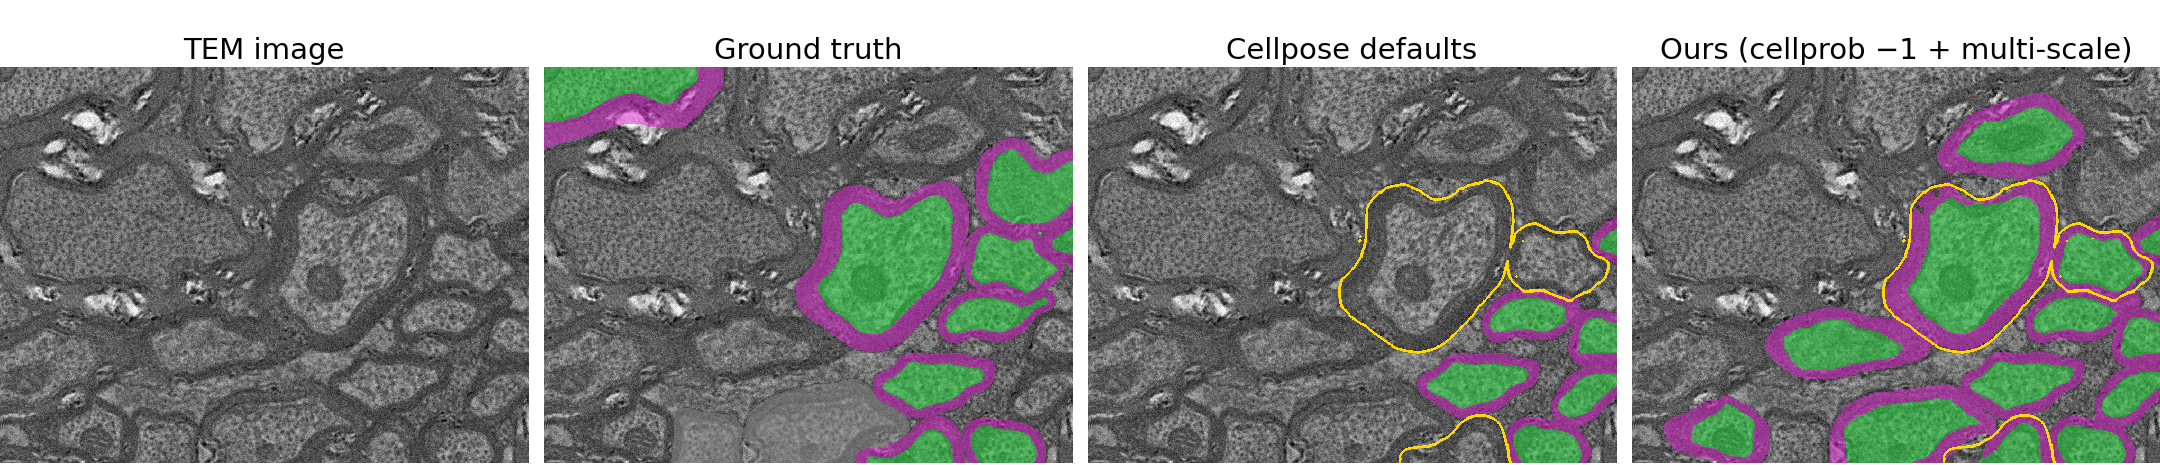
\includegraphics[width=\textwidth]{figures/qualitative.png}
\caption{Validation crop. Axons in green, myelin in magenta, artifact (ignored by
the metrics) in gray. Ground-truth fibers that only the proposed inference
recovers are outlined in yellow. The proposed inference also adds detections in
unannotated regions, a cost that Table~\ref{tab:oracle} shows to be small
compared with missed fibers.}
\label{fig:qualitative}
\end{figure*}

We first evaluated the models with the default Cellpose inference. Of the 1094
annotated validation fibers, 938 are matched (IoU $\geq0.5$) and 156 (14.3\%)
are missed; there are only 36 false positives on background (57 more lie
mostly inside artifact regions, which are not scored). The matched fibers are
accurate: their median IoU is 0.966 and their g-ratio bias is $-0.0009$.

Table~\ref{tab:oracle} corrects each error type with the ground truth. Removing
all false positives barely changes the HD95 (669 to 653~nm), and perfect
boundaries on the matched fibers mainly reduce MAE$_g$. Adding the missed fibers,
however, lowers the HD95 to 24~nm. Consistently, the HD95 is determined by the
ground-truth-to-prediction direction in 33/39 images for the axon and 30/39 for
the myelin, and 93\% of the farthest ground-truth boundary pixels belong to
missed fibers. Passing the ground truth through the $\times0.25$ downscaling and
upsampling yields a DSC of 0.986 and an HD95 of 4~nm, so working at reduced
resolution is not the bottleneck.

The missed fibers are entirely absent from the prediction and larger than the
detected ones (median area $1.44\times10^5$ vs.\ $0.96\times10^5$ pixels); 132
of the 156 are missed by the fiber model and 24 are lost because their axon is
not detected. Inside the fibers missed by the fiber model, the median predicted
cell probability is $-0.71$, against $3.40$ inside detected fibers, and it is
positive for 19\% of them: the network partially responds to these fibers but
remains below the default threshold. This behavior is not overfitting: on 12
training images the same models miss 12.4\% of the fibers and reach a DSC of
0.837, close to the validation figures. These observations motivate the
inference of Section~\ref{sec:inference}.

% =====================================================================
\section{Results}

Table~\ref{tab:results} compares inference settings for the same trained
models. Disabling the Cellpose flow-error check recovers few fibers and degrades
MAE$_g$, because it admits poorly shaped masks. Lowering the cell-probability
threshold or adding the half-scale pass each improve all three metrics; the
combination of both gives the best DSC for both compartments (0.865 on average,
+0.037), an HD95 of 535~nm ($-134$~nm) and the lowest MAE$_g$ (0.0151), and is
our final configuration. The half-scale pass alone gives a slightly lower HD95
(529~nm) at the cost of a higher MAE$_g$. Fig.~\ref{fig:qualitative} shows a
large fiber recovered by the proposed inference. The final configuration was
selected among the six settings of Table~\ref{tab:results} on the same
validation images, so its scores may be slightly optimistic.

% =====================================================================
\section{Discussion and Conclusion}

The error analysis shifts the focus from boundary accuracy to detection: the
matched fibers are already precise, and a model operating at one quarter of the
original resolution is not resolution-limited, whereas each missed fiber adds a
large, isolated ground-truth contour that dominates the HD95. A simple change at
inference, a lower probability threshold and a second, coarser scale, captures
part of this gap at no training cost, but most missed fibers are still not
detected (the HD95 remains 535~nm against 24~nm for the oracle). Because the
models behave similarly on training and validation images, their predictions
on the training set could supervise a second-stage detector of missed fibers;
training with wider scale augmentation is another direct remedy. Limitations of
this study are the single random validation split of 39 images, the use of
the same split for selecting the inference settings, and the treatment of
artifact regions as background during training.

In summary, two fine-tuned Cellpose-SAM models combined by construction give
valid paired axon/myelin instances, and a recall-oriented multi-scale inference
reaches a mean DSC of 0.865, an HD95 of 535~nm and an MAE$_g$ of 0.0151 on our
validation split. The code is provided with the submission.

\section*{Acknowledgment}
% TODO: agradecimientos / financiación
We thank the organizers of the TEM Axon \& Myelin Segmentation Challenge and the
Paris Brain Institute (ICM) for providing the annotated dataset.

\bibliographystyle{IEEEtran}
\bibliography{refs}

\end{document}
